\documentclass[10pt, a4paper,twoside]{report} 
%%%%%%%%       12pt, a4paper,twoside]{report}     Kanske ändra till 10?

\usepackage[utf8]{inputenc}        %%% På den egna datorn
%\usepackage[latin1]{inputenc}      %%% På INCA servern
%\usepackage{Sweave}




\usepackage{etex}
\usepackage{roboto}
\usepackage{datetime}
%\usepackage{fancyhdr}
\usepackage{hyperref}
\usepackage[dotinlabels]{titletoc}
\usepackage[titles]{tocloft}
\usepackage{lipsum}
\usepackage{blindtext}
\usepackage{anyfontsize}
\usepackage[pagestyles]{titlesec}									% Fixa layout på sectionnumber
%\usepackage{fancyhdr}
\usepackage{xcolor}
\usepackage[hang,labelsep=period, margin=1.5cm]{caption}

\titleformat{\chapter}[display]{\bfseries\sffamily\Huge\color{useblue}}{\bfseries\sffamily\fontsize{20}{25}\selectfont\color{useblue}\MakeUppercase{\chaptertitlename}{\sffamily\thechapter}}{-10 pt}{\bfseries\sffamily\fontsize{20}{25}\selectfont}
\titleformat{\section}{\bf\sffamily\color{useblue}\fontsize{16}{19}\selectfont}{\bf\sffamily\color{useblue}\fontsize{16}{19}\selectfont\thesection}{1em}{}
\titleformat{\subsection}{\bf\sffamily\color{useblue}\fontsize{14}{17}\selectfont}{\bf\sffamily\color{useblue}\fontsize{14}{17}\selectfont\thesubsection}{1em}{}
\titleformat{\subsubsection}{\bf\sffamily\color{useblue}\fontsize{10}{12}\selectfont}{\\bf\sffamily\color{useblue}\fontsize{10}{12}\selectfont\thesubsubsection}{1em}{}

\titlespacing\chapter{0pt}{0pt}{0pt}

\titlespacing\section{0pt}{0pt}{-4pt}
\titlespacing\subsection{0pt}{0pt}{-4pt}
\titlespacing\subsubsection{0pt}{0pt}{-4pt}

\renewcommand{\thesection}{\arabic{section}}
\usepackage[headsep=1.4cm, footskip = 1.4cm, top=2.5cm, bottom=2.5cm,outer=2.5cm,inner=3.0cm]{geometry} 
%%%%%%%%%   headsep=2.9cm, footskip = 1.9cm, top=4.0cm, bottom=3.0cm,outer=2.5cm,inner=3.0cm]{geometry}
\usepackage[swedish]{babel}
\usepackage[none]{hyphenat}
\usepackage{tikz}
\usepackage{pgf}
\usepackage{pdfpages}
\usepackage{datetime}
\newdateformat{usvardate}{%  
\MakeUppercase{\monthname} \THEYEAR}

%\usepackage[hang,labelsep=period]{caption}

\newcommand{\colemph}[1]{\textcolor{red}{#1}}

\renewcommand{\subsectionmark}[1]{\markboth{\textcolor{useblue}{\textsf{\fontsize{8pt}{12pt}\selectfont{\textbf{\thesubsection \hspace{2mm} #1}}}}}{}}



\newpagestyle{main}{%
    \sethead[\leftmark\begin{tikzpicture}[remember picture,overlay]\node[yshift=-1cm] at (current page.north east){\begin{tikzpicture}[remember picture, overlay]\fill[useblue] (-0.019\paperwidth,-0.4) circle (0.0438\paperwidth);\end{tikzpicture}};\end{tikzpicture}]
            []
            []
            {\begin{tikzpicture}[remember picture,overlay]\node[yshift=-1cm] at (current page.north west){\begin{tikzpicture}[remember picture, overlay]\fill[useblue] (0.019\paperwidth,-0.4) circle (0.0438\paperwidth);\end{tikzpicture}};\end{tikzpicture}}
            {}
            {\textcolor{useblue}{\textsf{\fontsize{8pt}{12pt}\selectfont{\textbf{ \MakeUppercase{\thesection\,\,\sectiontitle}}}}}}
    \setfoot[\textcolor{useblue}{\textsf{\fontsize{8pt}{12pt}\selectfont{\textbf{ \thepage \, | Tolkningsmanual för interaktiva Shinyrapporter \colemph{}}}}}]
            []
            []
            {}
            {}
            {\textcolor{useblue}{\textsf{\fontsize{8pt}{12pt}\selectfont{\textbf{ \colemph{} Tolkningsmanual för interaktiva Shinyrapporter | \thepage}}}}}
}

\newpagestyle{asdf}{%
    \sethead[\textcolor{useblue}{\textsf{\fontsize{8pt}{12pt}\selectfont{\textbf{ \uppercase{\thesection\,\,\sectiontitle}}}}}\begin{tikzpicture}[remember picture,overlay]\node[yshift=-1cm] at (current page.north east){\begin{tikzpicture}[remember picture, overlay]\fill[useblue] (-0.019\paperwidth,-0.4) circle (0.0438\paperwidth);\end{tikzpicture}};\end{tikzpicture}]
            []
            []
            {\begin{tikzpicture}[remember picture,overlay]\node[yshift=-1cm] at (current page.north west){\begin{tikzpicture}[remember picture, overlay]\fill[useblue] (0.019\paperwidth,-0.4) circle (0.0438\paperwidth);\end{tikzpicture}};\end{tikzpicture}}
            {}
            {\textcolor{useblue}{\textsf{\fontsize{8pt}{12pt}\selectfont{\textbf{ \MakeUppercase{\chaptername\,\thechapter \,\,\chaptertitle}}}}}}
    \setfoot[\textcolor{useblue}{\textsf{\fontsize{8pt}{12pt}\selectfont{\textbf{ \thepage \, | Tolkningsmanual för interaktiva Shinyrapporter \colemph{}}}}}]
            []
            []
            {}
            {}
            {\textcolor{useblue}{\textsf{\fontsize{8pt}{12pt}\selectfont{\textbf{ \colemph{} Tolkningsmanual för interaktiva Shinyrapporter | \thepage}}}}}
}


\let\origdoublepage\cleardoublepage
\newcommand{\clearemptydoublepage}{%
  \clearpage
  {\pagestyle{empty}\origdoublepage}%
}

\usepackage{etoolbox}

\usepackage{helvet}

% \usepackage{ebgaramond}
% \usepackage[sfdefault]{roboto}
\renewcommand{\familydefault}{\sfdefault}

\usepackage{xcolor}
% 
% \definecolor{RCCOrange}{HTML}{FFB117}
% \definecolor{RCCBlue}{HTML}{438DCC}
% \definecolor{RCCBlue}{HTML}{3ECAFF}
% \definecolor{RCCBlueDarker}{HTML}{009CD7}%{008FC6}%{FFFFFF}
% \definecolor{RCCLightBlue}{HTML}{3ECAFF}%{32C7FF}%{1FC1FF}
% \definecolor{RCCLightBlue}{HTML}{00B3F6}
% 
% \definecolor{rccblue}{HTML}{00B3F6}
% \definecolor{rccorange}{HTML}{FFB117}
\definecolor{useblue}{HTML}{005092}
% \definecolor{useblue}{HTML}{09528F}

%Lägger in 'luft' mellan meningar
\setlength{\parindent}{0pt}
\setlength{\parskip}{2ex plus 0.5ex minus 0.2ex}


\renewcommand{\familydefault}{\sfdefault}
\renewcommand{\familydefault}{\rmdefault}

\usepackage{float}

\floatplacement{table}{H}
\floatplacement{figure}{H}

\newenvironment{centerfig}
{\begin{figure}[H]\centering}
{\end{figure}}

\newenvironment{rotatetab}[2]
{\begin{table}[H]\footnotesize\centering\caption{#2}\label{#1}\begin{sideways}}
{\end{sideways}\end{table}}


    % En mapp Figurer ska ligga i målmappen. Här hamnar alla figurer
 

\usepackage{chngcntr} %%%%%%%% Tillagt för olika numrering av figurer i kapitel






\begin{document}
%\Sconcordance{concordance:Tolkningsmanual_Shinyrapporter.tex:Tolkningsmanual_Shinyrapporter.Rnw:%
1 351 1}

\pagestyle{empty}
     \includepdf[width=\paperwidth,pagecommand={
\begin{tikzpicture}[remember picture, overlay] 
     \fill[useblue] ([shift={(-0.055\paperwidth,-0.34\paperwidth)}]current page.north east) circle (0.14\paperwidth);
     \node at (7.0,-2.25) {%
     %%%%%%%  (7.0,-0.85) {%
     \parbox[t][8pt][t]{0.67\paperwidth}{%
     \roboto{\fontsize{36pt}{12pt}\selectfont{\textbf{Tolkningsmanual \\för interaktiva \\Shinyrapporter}}} \\[22pt]
     \roboto{\fontsize{18pt}{12pt}\selectfont{\textcolor{useblue}{}}} \\[45pt]
     \roboto{\fontsize{12pt}{12pt}\selectfont{november 2019   }} 
     %%%%%%%    ntsize{12pt}{12pt}\selectfont{november 2019   }} \\[6pt] 
     %\roboto{\fontsize{12pt}{12pt}\selectfont{Version: \#005092}}
     }%
     };
          \node at (7.0,-19.45) {%
     \parbox{0.67\paperwidth}{%
     % \textsf{\resizebox{\linewidth}{!}{\textbf {XXXXcancer}} %\\[12pt]
     %\roboto{\fontsize{12pt}{12pt}\selectfont{Här kan text rörande innehållet läggas}}
     }%
     };
     \node at ([shift={(-27mm,18mm)}]current page.south east){%
     
\includegraphics[width=0.16\paperwidth]{rccsam_logga_bw.png}
     };
     \end{tikzpicture}
     }]{rccsam_banner2[1].png}
%\newpage
%\mbox{}
%\vfill

%\begin{minipage}{\textwidth}
% Tar bort box runt klickbara länkar (href)
%\hypersetup{
%    colorlinks=false,
%    pdfborder={0 0 0},
%}

%\small
%
\includegraphics[width=6cm]{rccsam_logga_rgb.png} \newline
%\newline
%\sffamily Beställningsadress\newline
%\newline
%\sffamily Regionalt cancercentrum Norr \newline 
%\sffamily Norrlands universitetssjukhus \newline 
%\sffamily SE-901 85 UMEÅ \newline
%\newline
%\sffamily Tel\quad 090-785 19 90 \newline
%\newline
%\sffamily Mailadress - \href{mailto:rccnorr@vll.se}{\color{blue}{rccnorr@vll.se}}\newline
%\newline
%\sffamily Rapporterna kan laddas ner från \newline
%\sffamily \href{http://www.cancercentrum.se/norr/cancerdiagnoser/tjocktarm-andtarm-och-anal/tjock--och-andtarm/kvalitetsregister/rapporter/}{\color{blue}{rapporter}} \newline

%\vspace{1cm}
%\copyright\,2018 Regionalt cancercentrum Norr, Norra sjukvårdsregionen
%\normalsize
%\end{minipage}
%\clearemptydoublepage
%\thispagestyle{empty} 
%\renewcommand\contentsname{Innehållsförteckning}

% \newlength\mylength
% \renewcommand\cftchappresnum{\chaptername~}
% \renewcommand\cftchapaftersnum{\newline}
% \settowidth\mylength{\cftchappresnum\cftchapaftersnum\newline}
% \addtolength\cftchapnumwidth{\mylength}

\titlecontents{chapter}% <section-type>
  [0pt]% <left>
  {\bf\sffamily\fontsize{11pt}{13pt}\selectfont}% <above-code>
  {\chaptername\ \thecontentslabel:\newline}% <numbered-entry-format>
  {}% <numberless-entry-format>
  {\,\sf\sffamily\titlerule*[0.75pc]{.}\,\bf\sffamily\contentspage}% <filler-page-format>

\renewcommand{\cftchapfont}{\bf\sffamily\fontsize{11pt}{13pt}\selectfont}
\renewcommand{\cftchappagefont}{\bf\sffamily\fontsize{11pt}{13pt}\selectfont}
\renewcommand{\cftchapdotsep}{\cftdotsep}


\renewcommand{\cftsecleader}{\cftdotfill{\cftdotsep}}

\renewcommand{\cftsecfont}{\bf\sffamily\fontsize{11pt}{13pt}\selectfont}
\renewcommand{\cftsecpagefont}{\bf\sffamily\fontsize{9pt}{11pt}\selectfont}
%\setlength{\cftsecindent}{0em}

\renewcommand{\cftsubsecfont}{\sffamily\fontsize{11pt}{13pt}\selectfont}
\renewcommand{\cftsubsecpagefont}{\sffamily\fontsize{11pt}{13pt}\selectfont}
%\setlength{\cftsubsecindent}{0em}

\renewcommand{\cftsubsubsecfont}{\it\sffamily\fontsize{11pt}{13pt}\selectfont}
\renewcommand{\cftsubsubsecpagefont}{\it\sffamily\fontsize{11pt}{13pt}\selectfont}
%\setlength{\cftsubsubsecindent}{0em}

\renewcommand{\cfttabfont}{\sffamily}
\renewcommand{\cfttabpagefont}{\sffamily}

\renewcommand{\cftfigfont}{\sffamily}
\renewcommand{\cftfigpagefont}{\sffamily}
\pagenumbering{gobble}
\thispagestyle{empty}
\hypersetup{hidelinks}
\tableofcontents
\clearpage

\pagestyle{main}
\pagenumbering{arabic}
\setcounter{page}{1}
\patchcmd{\chapter}{\thispagestyle{plain}}{}{}{}
%\pretocmd{\chapter}{\pagestyle{asdf}\renewcommand{\thesection}{\thechapter.\arabic{section}}\clearemptydoublepage}{}{}
\pretocmd{\chapter}{\pagestyle{asdf}\renewcommand{\thesection}{\thechapter.\arabic{section}}}{}{}
\titleformat{\chapter}[display]{\sffamily\Huge\color{black}}{\sffamily\fontsize{30}{25}\selectfont\color{useblue}\MakeUppercase{\chaptertitlename}\hspace{1ex}{\sffamily\thechapter}}{-10 pt}{\bfseries\sffamily\fontsize{20}{10}\selectfont}
\titlespacing\chapter{0pt}{0pt}{25pt}
%%%%%%%%     \chapter{0pt}{96pt}{25pt}

\setkeys{Gin}{width=0.8\textwidth}     						% Deklarera hur stor bredd en figur får ta
\raggedbottom
\raggedright

%\chapter{testkapitel}

%För rapporter som publiceras på fler än ett språk görs det valet uppe i det vända hörnet.

%\setkeys{Gin}{width=0.15\textwidth}
%
\includegraphics[]{figurer/Sprakval}
%\newline

\section{Instruktioner för användande av de interaktiva shinyrapporterna}
Detta dokumentet är tänkt att vara till hjälp för användare av våra interaktiva årsrapporter (Shinyrapporter) som finns att hitta på \href{https://www.cancercentrum.se/samverkan/vara-uppdrag/statistik/kvalitetsregisterstatistik/interaktiva-rapporter/}{\color{blue}{cancercentrum.se/samverkan/vara-uppdrag/statistik/kvalitetsregisterstatistik/interaktiva-rapporter/}}. \newline
Figurerna som genereras i dessa rapporter kan sparas till din dator. Om du högerklickar på en figur så kan du välja ''Spara bild som'' och sedan spara figuren på din dator om du behöver använda den till t.ex. en presentation.

\section{Val av indikator}
När en interaktiv årsrapport öppnas finner du till att börja med en startsida. Där finns information från registret om rapporten. Du finner även en flikmeny högst upp på sidan under rubriken. Dessa flikar är kapitlen som finns i det aktuella registret.

\setkeys{Gin}{width=1\textwidth}

\includegraphics[]{figurer/Overmeny1}
\newline

När du klickar på en flik visas de indikatorer som finns i den filken i en undermeny. För att se en av dessa indikatorer klickar du på den och så ska figuren öppnas nedanför.

\setkeys{Gin}{width=1\textwidth}
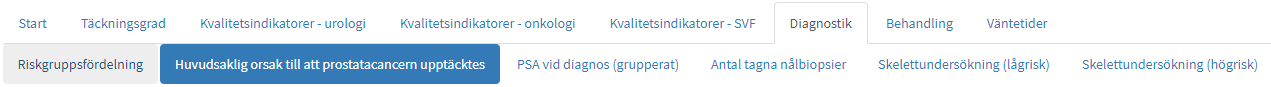
\includegraphics[]{figurer/Overmeny2}
\newline

\section{Urvalsdialog}
När du har öppnat en indikator kommer denna att visas under menyn. Du kommer då att se en figur till höger och till vänster finns en urvalsruta där du kan göra urval för den öppnade indikatorn. Om du ändrar ett urval så kommer figuren/tabellen att laddas om och den nya figuren/tabellen baseras på dina urval. Figurerna/tabellerna uppdateras i realtid direkt du ändrar något urval.

\setkeys{Gin}{width=0.6\textwidth}
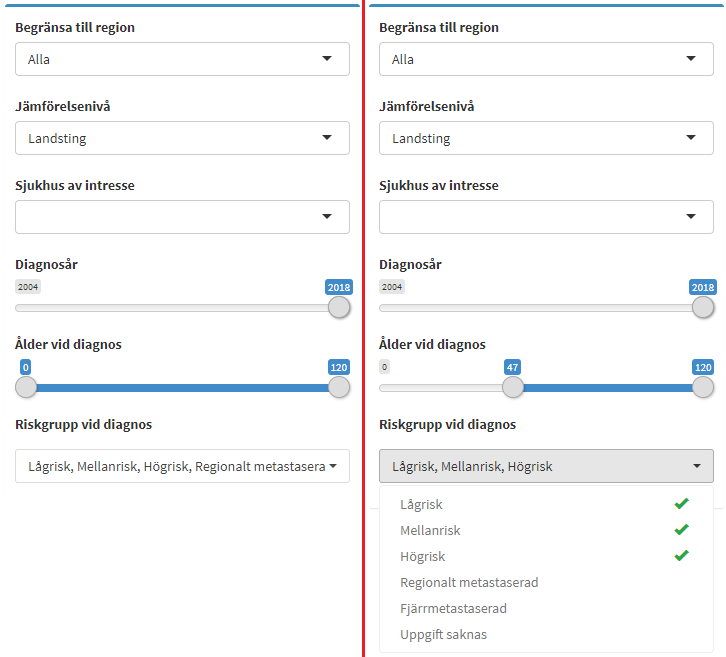
\includegraphics[]{figurer/Urvalsdialog_gemensam}
\newline

Under titeln för indikatorn återfinns de aktuella urvalen som är gjorda. Om urval på en variabel inte är gjort utan samtliga möjliga val är valda kommer denna variabel ej att stå i listan.

\setkeys{Gin}{width=0.6\textwidth}
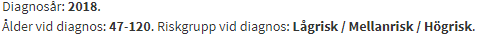
\includegraphics[]{figurer/Urvalstext}
\newline

\section{Resultat}
När du gjort dina urval finner du den uppdaterade indikatorn till höger. Det finns en meny där som kan se ut på lite olika sätt beroeden på vad för typ av indikator det är och vad registret valt att visa.

\setkeys{Gin}{width=0.8\textwidth}

\includegraphics[]{figurer/Grafval1}\newline
\setkeys{Gin}{width=0.68\textwidth}

\includegraphics[]{figurer/Grafval2}
\newline

Under \textcolor{useblue}{\fontfamily{phv}\selectfont{Jämförelse}} hittar du stapelfigurer. De är uppdelade på antingen Region, Sjukvårdsregion eller Sjukhus. Om registret valt att ha med fler än en jämförelsenivå kommer dessa att kunna väljas bland urvalen till vänster. Vad som visas beror på indikatorn. Det kan t.ex. vara antalet som fått en viss behandling eller fördelning av tumörstadium som så kallade stackade staplar. Om det är en ledtid kommer som standard mediantiden att visas men det kan även finnas möjlighet att välj att se andelen inom X dagar om registret valt att inkludera detta. \newline
Ett grönt skuggat område bakom staplarna betyder att registret har valt att ha en målnivå för indikatorn. Målet är uppnått om stapeln går över det det skuggade området. Ett gult skuggat område betyder att målnivån har 2 nivåer och det gula är ett lättare mål att uppnå.

\setkeys{Gin}{width=0.5\textwidth}
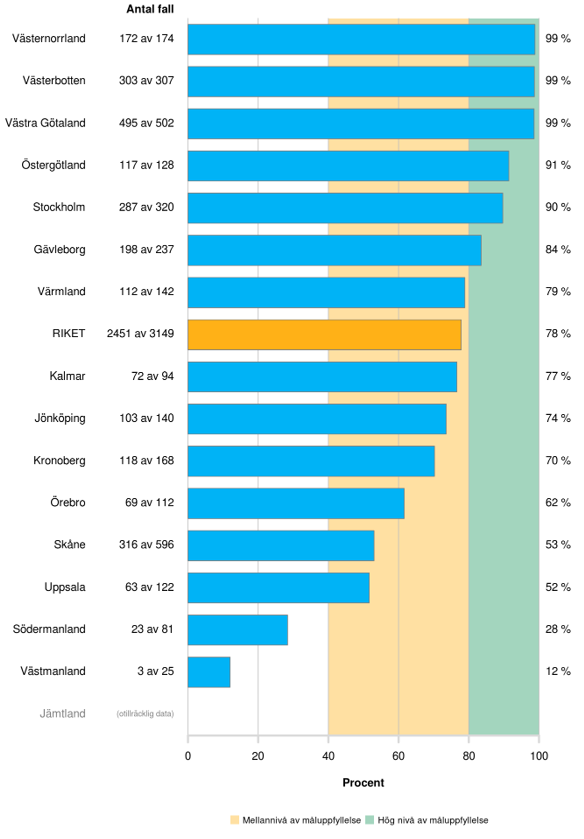
\includegraphics[]{figurer/Jamforelse1}
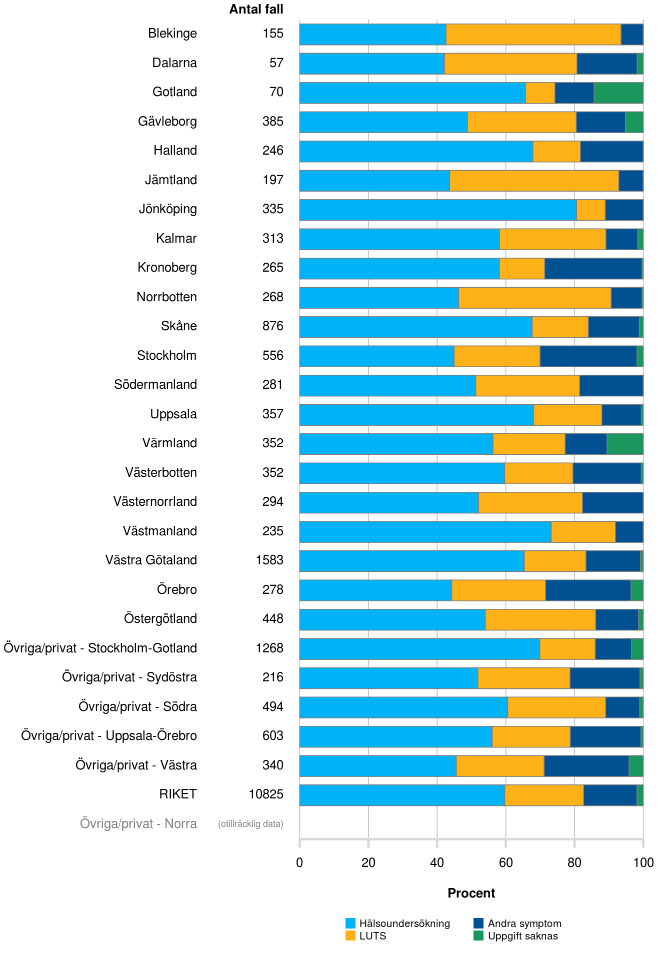
\includegraphics[]{figurer/Jamforelse2}
\newline

Under \textcolor{useblue}{\fontfamily{phv}\selectfont{Tabell}}, \textcolor{useblue}{\fontfamily{phv}\selectfont{Tabell (Antal)}} och \textcolor{useblue}{\fontfamily{phv}\selectfont{Tabell (Andel)}} hittar du tabeller över de data som presenteras i Jämförelse-fliken. Vilken/Vilka av de 3 tabell-flikarna som visas beror på vad det är för typ av indikator. Via kapparna i tabellerna kan antalssiffrona hämtas hem i lite olika format, Excel, PDF, eller i utskriftsformat.

\setkeys{Gin}{width=1\textwidth}
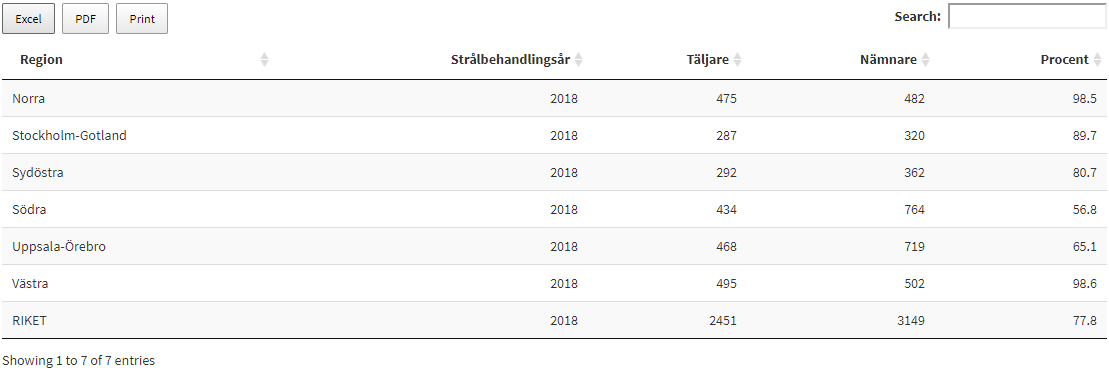
\includegraphics[]{figurer/Tabell}
\newline
\clearpage

Under \textcolor{useblue}{\fontfamily{phv}\selectfont{Trend}} hittar du trender över per år över data enligt dina urval (du får dock alltid samtliga år här). Hur trenderna ser ut beror på vad det är för typ av didikator som du tittar på. För kategoriska indikatorer, som t.ex. fördelning av tumörstadium, är trenderna rikets siffror. Du kan då också välja att visa trendkurvan för ett specifikt sjukhus, län eller region. \newline
För indikatorer som t.ex. andel som fått en viss typ av behandling kommer trenderna vara över andelar för sjukvårdsregionerna samt riket. Här kan du även lägga till ett specifikt sjukhus trendkurva om registret presenterar data på sjukhusnivå.

\setkeys{Gin}{width=0.5\textwidth}
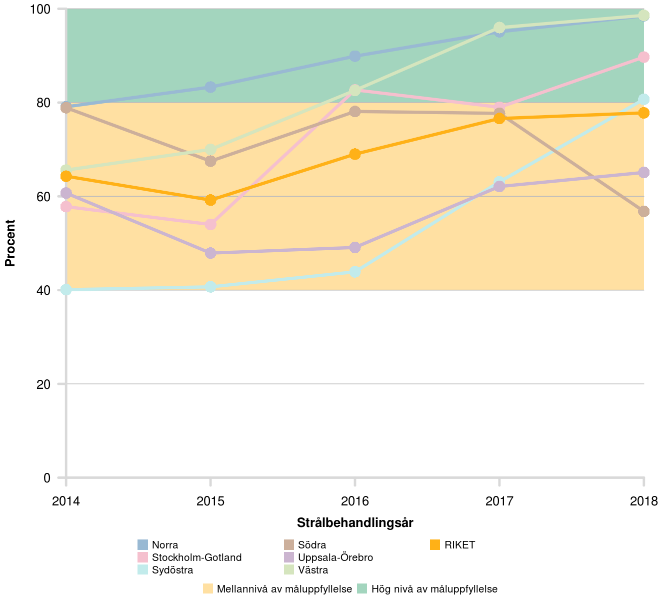
\includegraphics[]{figurer/Trend1}
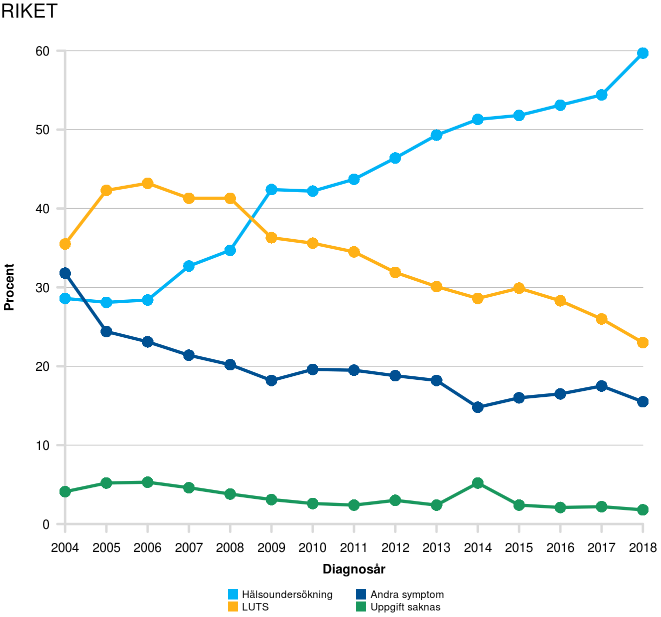
\includegraphics[]{figurer/Trend2}
\newline
\clearpage

Under \textcolor{useblue}{\fontfamily{phv}\selectfont{Karta}} hittar du indikatorn på kartform, denna finns endast med om landsting är en av jämförelsenivåerna och figuren inte är en så kallad stackad stapel. Län som är gråa har ej tillräckligt med data för att visa resultatet.

\setkeys{Gin}{width=0.5\textwidth}
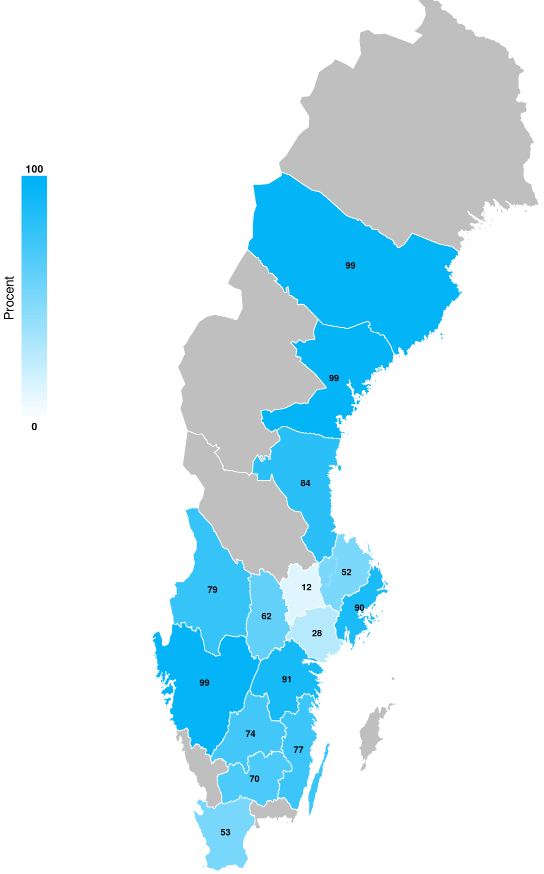
\includegraphics[]{figurer/Karta}
\newline
\clearpage

Under \textcolor{useblue}{\fontfamily{phv}\selectfont{Beskrivning}} hittar du information om indikatorn. Där kan du hitta 3 underrubriker, Om indikatorn, Att tänka på vid tolkning samt Teknisk beskrivning. Om du har någon fundering kring en indikator kan du titta här för att förhoppningsvis få svar på din fundering.

\setkeys{Gin}{width=1\textwidth}
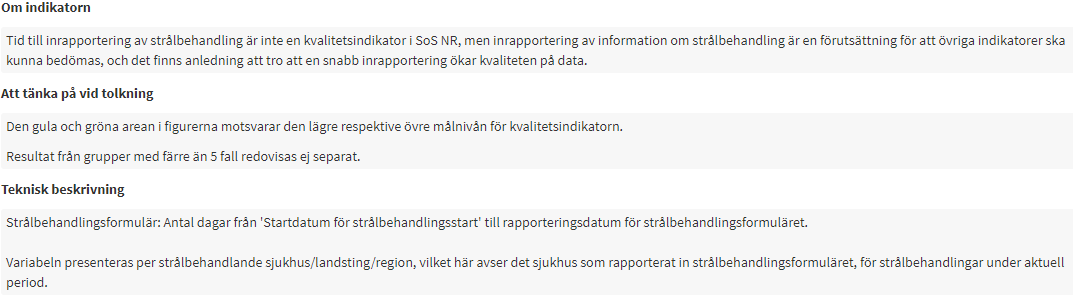
\includegraphics[]{figurer/Beskrivning}
\newline


\end{document}
